% -----------------------------------------------------------------
% Document class: Article
\documentclass[ a4paper, twoside, 11pt]{article}
\usepackage{../../macros-general}
\usepackage{../../macros-article}
% Number of the handout, quiz, exam, etc.
\newcommand{\numero}{01}
\setcounter{numero}{\numero}

% -----------------------------------------------------------------
\begin{document}
\allowdisplaybreaks

\begin{center}
\Large Sistemas de Control (EYAG-1005): Taller \numero \\[1ex]
\small \textbf{Semestre:} 2017-2018 T\'ermino I \qquad
\textbf{Instructor:} Luis I. Reyes Castro
\end{center}
\halfskip

Integrantes del Grupo:
\fullskip
\fullskip
\fullskip

% -----------------------------------------------------------------
\begin{problem}
Para el sistema mostrado en la figura de abajo, encuentre: 
\begin{itemize}
\item \textbf{[2 Puntos]} La funci\'on de transferencia en circuito cerrado $T(s) = C(s) / R(s)$. 
\item \textbf{[2 Puntos]} La tasa de amortiguamiento, el porcentage de sobrepaso, el tiempo pico y el tiempo de asentamiento. 
\end{itemize}

\begin{figure}[htb]
\centering
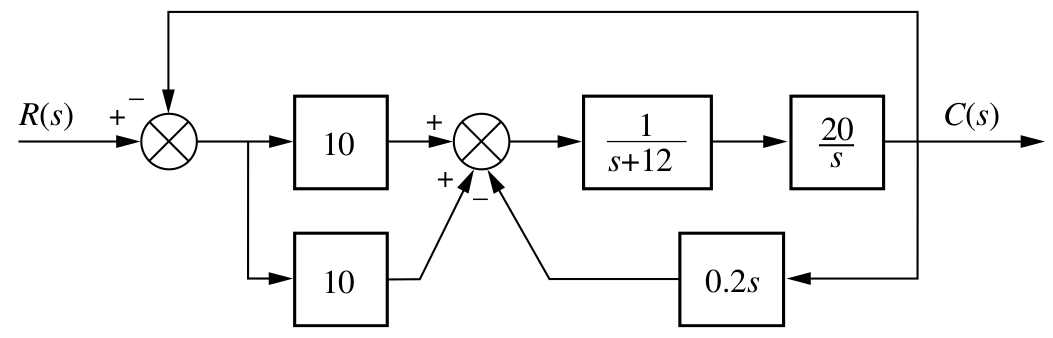
\includegraphics[width=0.64\columnwidth]{Nise_Prob-5-17.jpg}
\end{figure}

\emph{Soluciones:}
\begin{itemize}
\item \emph{Literal (i):}
\[
T(s) \; = \; \frac{400}{ s^2 + 16 \, s + 400 }
\]
\item \emph{Literal (i):} Dado que $\omega_n^2 = 400$ tenemos que $\omega_n = 20$. A su vez: 
\[
2 \, \zeta \omega_n \, = \, 16 \quad \Longrightarrow \quad \zeta \, = \, 0.4
\]
Consecuentemente:
\begin{align*}
OS \; 
& = \; \exp \left( -\frac{\zeta \, \pi}{\sqrt{1 - \zeta^2}} \right) \; = \; 0.2538 \; \equiv \; 25.38\% \\[1ex]
T_p \; 
& = \; \frac{\pi}{ \omega_n \, \sqrt{1 - \zeta^2}} \; = \; 0.1714 \, \text{seg} \\[1ex]
T_s \; 
& = \; \frac{4}{\zeta \, \omega_n} \; = \; 0.5 \, \text{seg}
\end{align*}
\end{itemize}

\end{problem}
\fullskip

% -----------------------------------------------------------------
\begin{problem}
En el 2014 el destructor estadounidense \emph{U.S.S. Ponce} demostr\'o exitosamente, por primera vez en la historia, el uso de un l\'aser de alta energ\'ia para detener un blanco m\'ovil. Con esto en mente, especulemos sobre el funcionamiento del sistema de gu\'ia del l\'aser a bordo del \emph{U.S.S. Ponce}. La mayor\'ia de destructores estadounidenses cuentan con grandes radares de apertura sint\'etica, asi que supondremos que un radar de este tipo es usado para guiar al l\'aser. (Un radar de apertura sint\'etica est\'a f\'isicamente sujeto a la estructura de su veh\'iculo portador y por lo tanto no necesita girar.) Supondremos tambi\'en que: 
\begin{itemize}
\item Cuando se desea apuntar el l\'aser hacia un potencial blanco el radar de apertura sint\'etica genera un \'angulo $\theta_r(t)$ que se utiliza como referencia para el \'angulo del l\'aser $\theta(t)$. 
\item El lazo de control tiene arquitectura de retro-alimentaci\'on unitaria con compensaci\'on delantera. Es decir, en cada instante se calcula el error angular $\theta_e(t) = \theta_r(t) - \theta(t)$ y se ingresa esa se\~nal a un compensador con funci\'on de transferencia $G_C(s)$ que genera el voltage que alimenta al motor el\'ectrico. 
\item El l\'aser es actuado por un motor el\'ectrico que genera un torque $T(t)$ sobre su estructura de 10 N-m por cada voltio de entrada. 
\item El momento de inercia de la estructura del l\'aser es de $J = 280$ kg-m\tsup{2} y el torque generado por la fricci\'on de la misma es de $K_f = 8.5$ N-m/(grado/s). 
\end{itemize}

Con esto en mente, suponga que usted fue el ingeniero encargado del dise\~no del sistema de gu\'ia del l\'aser y complete cada una de las siguientes actividades: 
\begin{itemize}
\item \textbf{[2 Puntos]} Bosqueje el lazo de control del sistema de gu\'ia del l\'aser. 
\item \textbf{[2 Puntos]} Suponga que el almirantazgo estadounidense especific\'o que el l\'aser debe ser capaz de ``apuntarle a embarcaciones enemigas navengando a velocidades de hasta 50 nudos a distancias de no menos de 1 milla n\'autica del destructor con un error no mayor a 5 milimetros''. Dise\~ne el compensador $G_C(s)$ m\'as sencillo capaz de alcanzar esta especificaci\'on. 
\item \textbf{[2 Puntos]} Suponga que el almirantazgo estadounidense especific\'o que el l\'aser debe ser capaz de ``apuntarle a aeronaves enemigas volando a cualquier velocidad con aceleraciones de hasta 2 nudos por segundo a distancias de no menos de 1 milla n\'autica del destructor con un error no mayor a 2 centimetros''. Dise\~ne el compensador $G_C(s)$ m\'as sencillo capaz de alcanzar esta especificaci\'on. 
\end{itemize}

\emph{Soluciones:}
\begin{itemize}
\item \emph{Literal (i):} De la descripci\'on del problema, si denotamos al voltage de entrada del motor el\'ectrico como $v(t)$ entonces podemos ver que la ecuaci\'on diferencial que gobierna el movimiento de la estructura del l\'aser es: 
\[
280 \, \ddot{\theta}(t) \; = \; 10 \, v(t) - (8.5)(180/\pi) \, \dot{\theta}(t)
\]
Por lo tanto la funci\'on de transferencia de la planta es: 
\[
G_P(s) \; = \; \frac{\Theta(s)}{V(s)} \; = \;
\frac{10}{ 280 \, s^2 + 487 \,s } \; = \; \frac{0.0357}{ s \, ( s + 1.74 )}
\]
Finalmente, la figura de abajo muestra el lazo de control del sistema. 
\begin{figure}[htb]
\centering
\def\svgwidth{0.8\columnwidth}
\input{fig_lazo-de-control.eps_tex}
\end{figure}

\item \emph{Literal (ii):} Primero interpretamos la se\~nal de referencia. Para esto obseramos que: 
\[
\dot{\theta_r}(t) \; = \; 
\frac{50 \, \text{nudos}}{1 \, \text{milla n\'autica}} \; = \; 
\frac{25.72 \, \text{m/s}}{1852 \, \text{m}} \; = \; 0.0139 \, \text{rad/s}
\]
Esto implica que la se\~nal de referencia es una rampa; m\'as precisamente: 
\[
\theta_r(t) \; = \; 0.0139 \, t
\]
Luego, el m\'aximo error permitido es: 
\[
e(\infty) \; = \; \frac{5 \, \text{mm}}{1 \, \text{milla n\'autica}} \; = \; \frac{0.005}{1852} \; = \; 2.7 \times 10^{-6}
\]
Ahora, puesto que la entrada es una rampa y que deseamos alcanzar un error en estado estable finito con respecto a esa entrada rampa, nuestro sistema debe de ser del Tipo I, \ie debe tener un integrador en el lazo. Como la planta ya tiene un integrador, el compensador m\'as sencillo capaz de alcanzar la especificaci\'on es un simple amplificador, \iec
\[
G_C(s) \; = \; K
\]
Para un sistema Tipo I el error en estado estable es el rec\'iproco de la constante de velocidad $K_v$. Para nuestro sistema tenemos que: 
\[
K_v \; = \; \lim_{ s \rightarrow 0 } \, s \, G_C(s) \, G_P(s)
\; = \; \frac{0.0357 \, K}{s + 1.74}
\]

\end{itemize}

\end{problem}
\vspace{\baselineskip}

\end{document}
